\documentclass[11pt,a4paper]{article}

\usepackage[parfill]{parskip}
\usepackage{subfig}
\usepackage{amsmath}
\usepackage{makeidx}
\usepackage{graphicx}
\usepackage[bibstyle=numeric, citestyle=numeric-comp]{biblatex}
\usepackage{multicol}
\usepackage{letltxmacro}

%\addbibresource[location=remote]{C:/Users/CptProton/Documents/Bibliographies/Labs.bib}

\LetLtxMacro{\oldsqrt}{\sqrt} % makes all sqrts closed
\renewcommand{\sqrt}[1][]{%
  \def\DHLindex{#1}\mathpalette\DHLhksqrt}
\def\DHLhksqrt#1#2{%
  \setbox0=\hbox{$#1\oldsqrt[\DHLindex]{#2\,}$}\dimen0=\ht0
  \advance\dimen0-0.2\ht0
  \setbox2=\hbox{\vrule height\ht0 depth -\dimen0}%
  {\box0\lower0.71pt\box2}}

\makeatletter
\newenvironment{tablehere}
  {\def\@captype{table}}
  {}

\newenvironment{figurehere}
  {\def\@captype{figure}}
  {}
\makeatother

\title{Automatic Fingerprint Recognition}
\author{Benjamin May \& Edward Wastell}
%\date{}

\begin{document}
\maketitle

\begin{abstract}
Stuff happened.
\end{abstract}

\begin{multicols}{2}

\section{Introduction}
	Fingerprints have been used to identify people since the 19\textsuperscript{th} century and have been used in criminal investigations since about that time. More recently fingerprints have been used as biometric markers used in boarder control, library stock control and computer and building access control systems. The need for a robust automatic fingerprint recognition system is obvious.

	Most fingerprint recognition systems in use are based on the idea of identifying minutiae (points where a ridge ends or joins with another ridge) --- in this article a system that uses the greylevel gradient to find minutiae is discussed.

\section{Theory}

	\subsection{Point Normal Determination}
\begin{figure*}
\centering
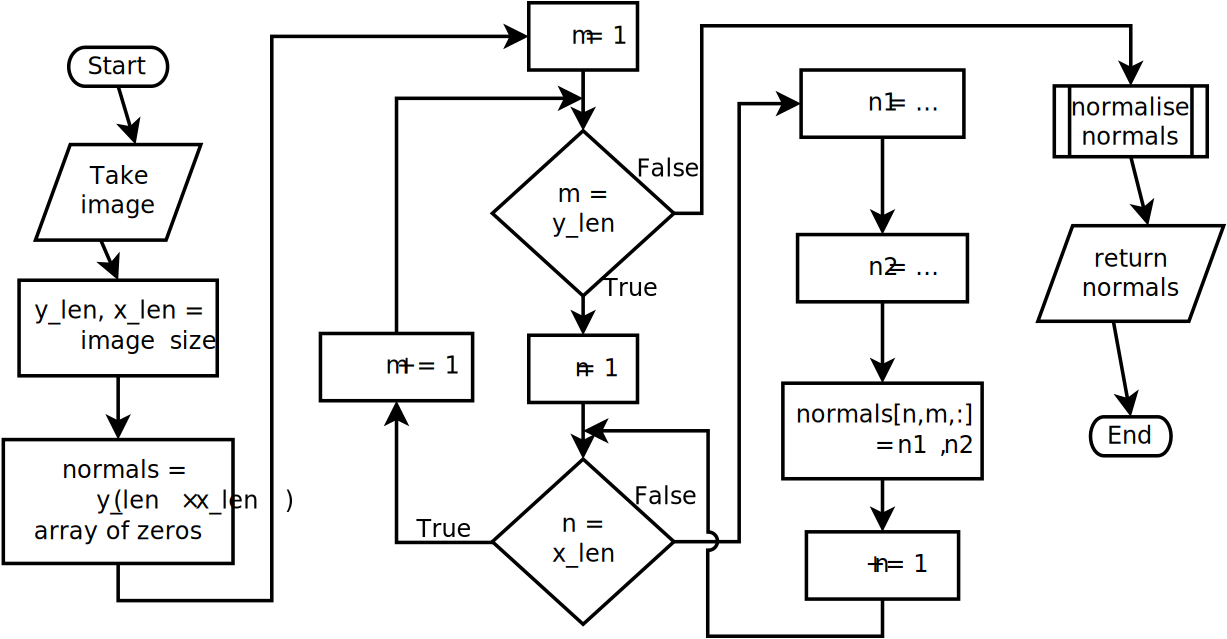
\includegraphics[width = \textwidth]{PND}
\caption{Flow chart of the PND function as implemented.}
\label{fig:PND-alg}
\end{figure*}

		The point normal function works by taking four mutually adjacent points (\textit{i.e.} a $2 \times 2$ array of pixels) and fitting a plane to them. The algorithm applied here (figure \ref{fig:PND-alg}) finds the planr with the minum 

\section{Experimental Procedure}

\section{Results \& Analysis}

\section{Conclusion}


\printbibliography

\end{multicols}

\end{document}
